\section{}
\textbf{Largest Connected Component: } 7659 nodes

\begin{figure}[h!]
    \begin{center}
        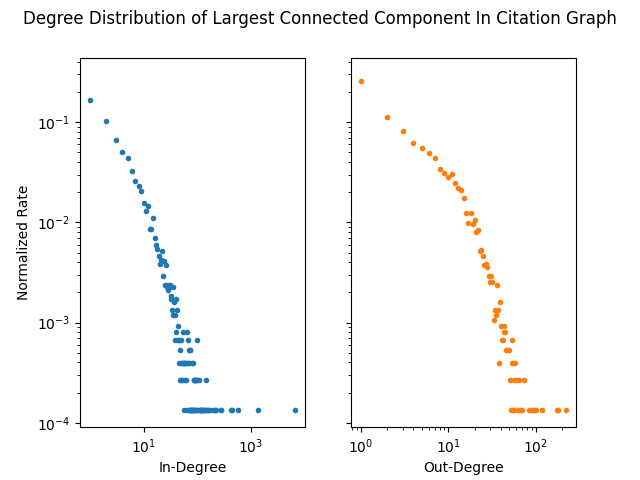
\includegraphics[width=.9\textwidth]{Q1-citations.png}
        \caption{Q1 - Degree Distribution of Largest Connected Component In Citation Graph}
        \label{fig:Q1}
    \end{center}
\end{figure}

\section{}
In short, the model has been adapted so that the out-degree of each node is now variable rather than fixed.
The out-degree is calculated by making a random selection of the out degrees of all existing nodes (during the incremental graph build process).
This adaption allows us to fairly accurately model the graph from Q1.
One of the limitations of this model is that there are fewer nodes with smaller degrees than the graph in Q1, hence visually we can see a more bottom heavy degree distribution graph in Figure \ref{fig:Q2}. 
\begin{figure}[h!]
    \begin{center}
        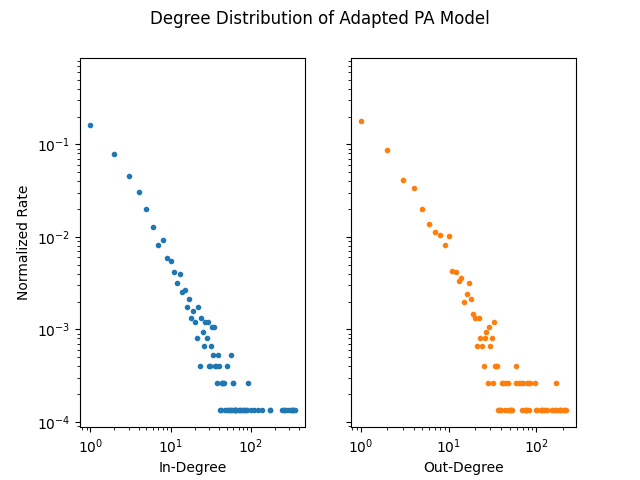
\includegraphics[width=.9\textwidth]{Q2.png}
        \caption{Q2 - Degree Distribution of Adapted PA Model}
        \label{fig:Q2}
    \end{center}
\end{figure}